In this chapter we explain the process of loading individual levels in our
game. This involves loading the level - encoded as an image in the PNG format -
parsing values from this format, and finally placing tiles in the game world
representing those values.

\section{Designing and loading levels}
Early in the development process, we established that for the type of game we
are making, it is important that we can quickly create levels with different
layout and sizes, for various reasons, such as:
\begin{itemize}
    \item Our development process, in it being agile. This should afford quick
        turnarounds and iterations, therefore requiring that we can quickly
        produces content for our game, such as levels.
    \item Game balancing, requiring us to produce levels at a sufficient pace in
        order to quickly iterate on game balancing topics, such as strategies
        for a particular map layout.
    \item That we do not have a dedicated level designer on our team, whom we
        could allocate to finely tune and manually design levels.
\end{itemize}

From the above arguments, it is clear that we not only want to produce levels
in a quick manner, but also automate the process of placing
\texttt{gameobjects} in the gameworld. While Unity's Editor can for many purposes
be thought of as a \textit{level editor}, we have chosen \textit{not} to use it
for designing levels for the following reasons:
\begin{itemize}
    \item Manually designing levels and placing gameobject in the Editor does
        not afford quick iterations, as required by our development process.
    \item The Editor does not afford easy refactoring of large levels, in that
        objects must be moved or replaced by hand. \textit{Large} is relative,
        but for our purposes it could be upwards +10.000 gameobjects.
    \item Individual levels would have to reside in individual \texttt{Scene}
        files, increasing the complexity of collaboration since scenefiles do
        not merge well in VCSs.
    \item A additional combinatorial complexity is introduced if we decide to
        also support different graphical appearances for objects in a level -
        what one could refer to as \textit{texture packs}. We would have
        to place a gameobject layout for each level for each texture pack.
\end{itemize}

While there are different approaches for circumventing the above
inconveniences, our solution is to encode the layout of each individual level
in an external file which is then loaded and interpreted. Historically, game
developers have often used this approach, usually encoded in some in-house
binary format. While we could have specified our own format, we have chosen to
encode the map in the PNG (Portable Network Graphics) for the following
reasons:
\begin{itemize}
    \item The PNG format is ubiquitous, in that there exists support for it
        almost anywhere, including in Unity3d - both in terms of API and the
        editor itself.
    \item It being ubiquitous means that we do not have to develop additional
        software in order to edit levels - most mainstream image editors
        support the PNG format.
    \item The PNG allows us to encode \textit{enough} information.
        \textit{Enough} being relative, but each colorchannel for each
        individual pixel offers 1 \texttt{byte} of information. With each pixel
        being encoded with RGBA (red, green, blue and alpha) channels, that
        gives us a total of 4 \texttt{bytes} of information, for each pixel.
\end{itemize}

Using the PNG format, it is then only a matter of specifying \textit{what} a
particular color should encode and interpreting that color when loading a
level. As an example, the following could specify how colors could be specified
to encode information about a level:
\begin{itemize}
    \item Black would be ground,
    \item green is grass,
    \item red is building floor, and
    \item yellow being building walls.
\end{itemize}

One obvious shortcoming from the above example is the lack of variation - maybe
one would like to be able to specify different types of walls or floors. This
could however be mitigated by either specifying more colors, by interpreting a
color randomly over a set or by interpreting a color differently depending on
the colors around it. To introduce variety into our levels, we use the latter
approach for some colors, which we will describe later in this chapter.
\\

Having decided on the format and encoded color values, we can design levels
such as seen in figure~\ref{fig:png_map}.

\begin{figure}[H]
    \centering
    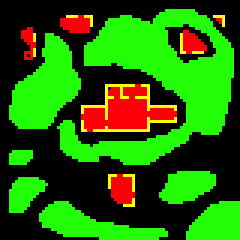
\includegraphics{figures/generating_levels/map.png}
    \caption{A PNG image encoding a map}\label{fig:png_map}
\end{figure}

From figure~\ref{fig:png_map}, we can immediately see that there are some
patches of grass, a building in the middle of the map and some torn-down
buildings in the periphery of the map. Some individual pixels of cyan color can
be seen, which encode where monster should appear. Likewise, a single white
pixel encode the exit point of the map, which is where players are required to
go to when the missions for this map have been completed. And last, a single
blue pixels encodes where the crafting table should be placed within the level.
\\
\\
Color values are then interpreted into distinct integer values in a
two-dimensional array, as seen in figure~\ref{fig:png_to_array}.
%thread carefully below...
\begin{figure}[H]
    \centering
    \begin{tabular}{cc}
        {\footnotesize
            \setlength{\tabcolsep}{4.5pt}
            \begin{tabular}{|c|c|c|c|c|c|c|c|c|c|}
                \hline
                \cellcolor{black} & \cellcolor{black} & \cellcolor{black} &
                \cellcolor{black} & \cellcolor{black} & \cellcolor{red} &
                \cellcolor{red} & \cellcolor{red} & \cellcolor{red} &
                \cellcolor{red} \\ \hline
                \cellcolor{green} & \cellcolor{green} & \cellcolor{black} &
                \cellcolor{black} & \cellcolor{black} & \cellcolor{yellow} &
                \cellcolor{red} & \cellcolor{red} & \cellcolor{red} &
                \cellcolor{red} \\ \hline
                \cellcolor{green} & \cellcolor{green} & \cellcolor{green} &
                \cellcolor{black} & \cellcolor{black} & \cellcolor{yellow} &
                \cellcolor{red} & \cellcolor{red} & \cellcolor{red} &
                \cellcolor{red} \\ \hline
                \cellcolor{green} & \cellcolor{green} & \cellcolor{green} &
                \cellcolor{black} & \cellcolor{black} & \cellcolor{yellow} &
                \cellcolor{red} & \cellcolor{red} & \cellcolor{red} &
                \cellcolor{red} \\ \hline
                \cellcolor{green} & \cellcolor{green} & \cellcolor{green} &
                \cellcolor{black} & \cellcolor{black} & \cellcolor{yellow} &
                \cellcolor{yellow} & \cellcolor{red} & \cellcolor{red} &
                \cellcolor{yellow} \\ \hline
                \cellcolor{green} & \cellcolor{green} & \cellcolor{green} &
                \cellcolor{black} & \cellcolor{black} & \cellcolor{black} &
                \cellcolor{black} & \cellcolor{black} & \cellcolor{black} &
                \cellcolor{black} \\ \hline
                \cellcolor{green} & \cellcolor{green} & \cellcolor{green} &
                \cellcolor{green} & \cellcolor{black} & \cellcolor{black} &
                \cellcolor{black} & \cellcolor{black} & \cellcolor{black} &
                \cellcolor{black} \\ \hline
                \cellcolor{green} & \cellcolor{green} & \cellcolor{green} &
                \cellcolor{green} & \cellcolor{black} & \cellcolor{black} &
                \cellcolor{black} & \cellcolor{black} & \cellcolor{black} &
                \cellcolor{black} \\ \hline
                \cellcolor{green} & \cellcolor{green} & \cellcolor{green} &
                \cellcolor{green} & \cellcolor{green} & \cellcolor{black} &
                \cellcolor{black} & \cellcolor{black} & \cellcolor{black} &
                \cellcolor{black} \\ \hline
                \cellcolor{green} & \cellcolor{green} & \cellcolor{green} &
                \cellcolor{green} & \cellcolor{green} & \cellcolor{green} &
                \cellcolor{green} & \cellcolor{green} & \cellcolor{green} &
                \cellcolor{black} \\ \hline
            \end{tabular}
        }
        &
        {\footnotesize
            \setlength{\tabcolsep}{2.5pt}
            \begin{tabular}{|c|c|c|c|c|c|c|c|c|c|}
                \hline
                0 & 0 & 0 & 0 & 0 & 4 & 4 & 4 & 4 & 4 \\ \hline
                1 & 1 & 0 & 0 & 0 & 3 & 4 & 4 & 4 & 4 \\ \hline
                1 & 1 & 1 & 0 & 0 & 3 & 4 & 4 & 4 & 4 \\ \hline
                1 & 1 & 1 & 0 & 0 & 3 & 4 & 4 & 4 & 4 \\ \hline
                1 & 1 & 1 & 0 & 0 & 3 & 3 & 4 & 4 & 3 \\ \hline
                1 & 1 & 1 & 0 & 0 & 0 & 0 & 0 & 0 & 0 \\ \hline
                1 & 1 & 1 & 1 & 0 & 0 & 0 & 0 & 0 & 0 \\ \hline
                1 & 1 & 1 & 1 & 0 & 0 & 0 & 0 & 0 & 0 \\ \hline
                1 & 1 & 1 & 1 & 1 & 0 & 0 & 0 & 0 & 0 \\ \hline
                1 & 1 & 1 & 1 & 1 & 1 & 1 & 1 & 1 & 0 \\ \hline
            \end{tabular}
        }
    \end{tabular}
    \caption{Interpreting a PNG map image into a two-dimensional array}\label{fig:png_to_array} 
\end{figure}

Values are then further separated into two-dimensional arrays consisting of
only each individual value.  The data within those arrays are what we use to
generate tiles and some game entities within the gameworld.

\section{Generating level backdrop}
As explained previously, our game is a top-down 2D action game. Important to
note is the top-down 2D aspect of it when we are to generate our levels.
A historical and still prevalent technique for 2D games, is using a
tiling approach for the layout of both the backdrop of the level and entities
within it. Several different approaches to tiling have been used in games,
including squares, isometric and hexagonal tiles.
Figures~\ref{fig:civ-1_square},~\ref{fig:civ-2_iso}~and~\ref{fig:wesnoth_hex}
show examples of games using each of the mentioned techniques of
tiling.

\begin{figure}[H]
    \centering
    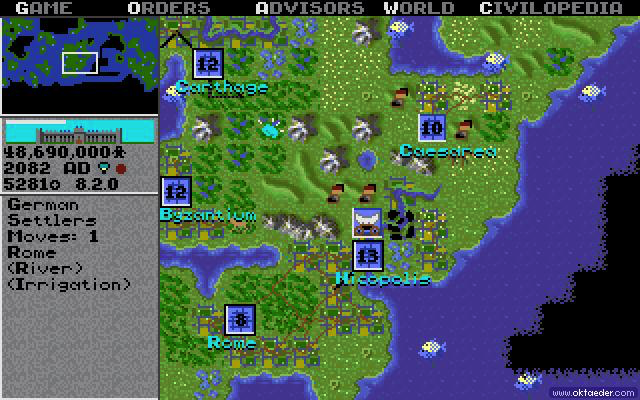
\includegraphics[width=1\textwidth]{figures/generating_levels/civ-1_square.png}
    \caption{Civilizations 1, using squares as tiles}\label{fig:civ-1_square} 
\end{figure}

\begin{figure}[H]
    \centering
    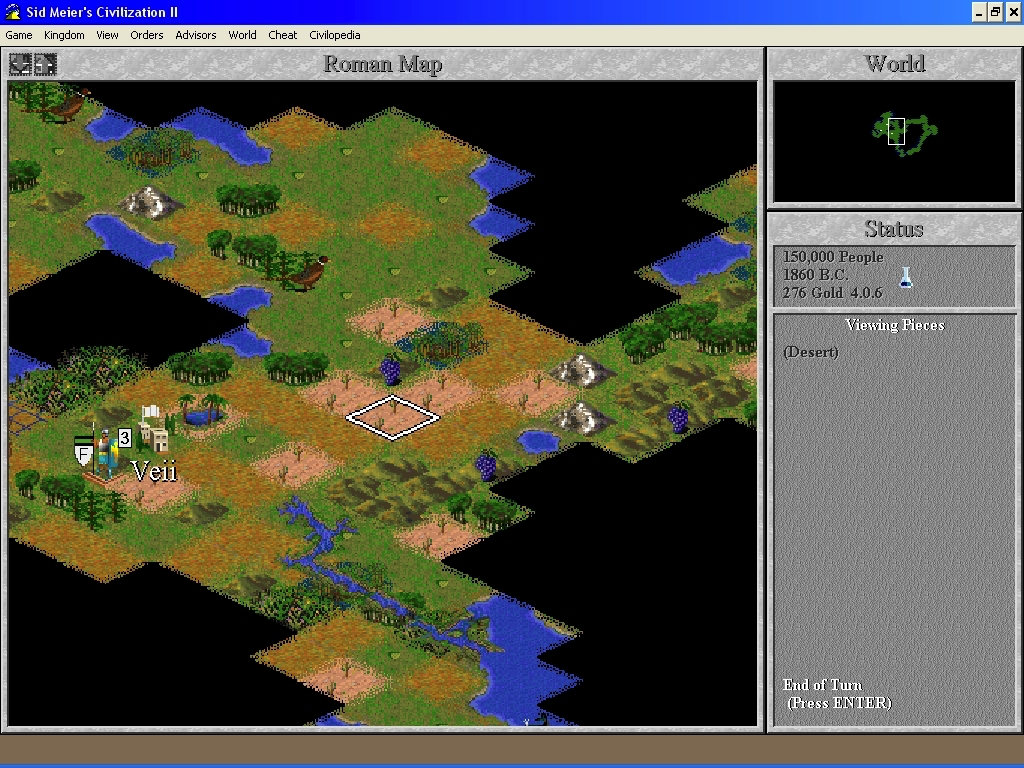
\includegraphics[width=1\textwidth]{figures/generating_levels/civ-2_iso.png}
    \caption{Civilizations 2, using the isometric technique}\label{fig:civ-2_iso} 
\end{figure}

\begin{figure}[H]
    \centering
    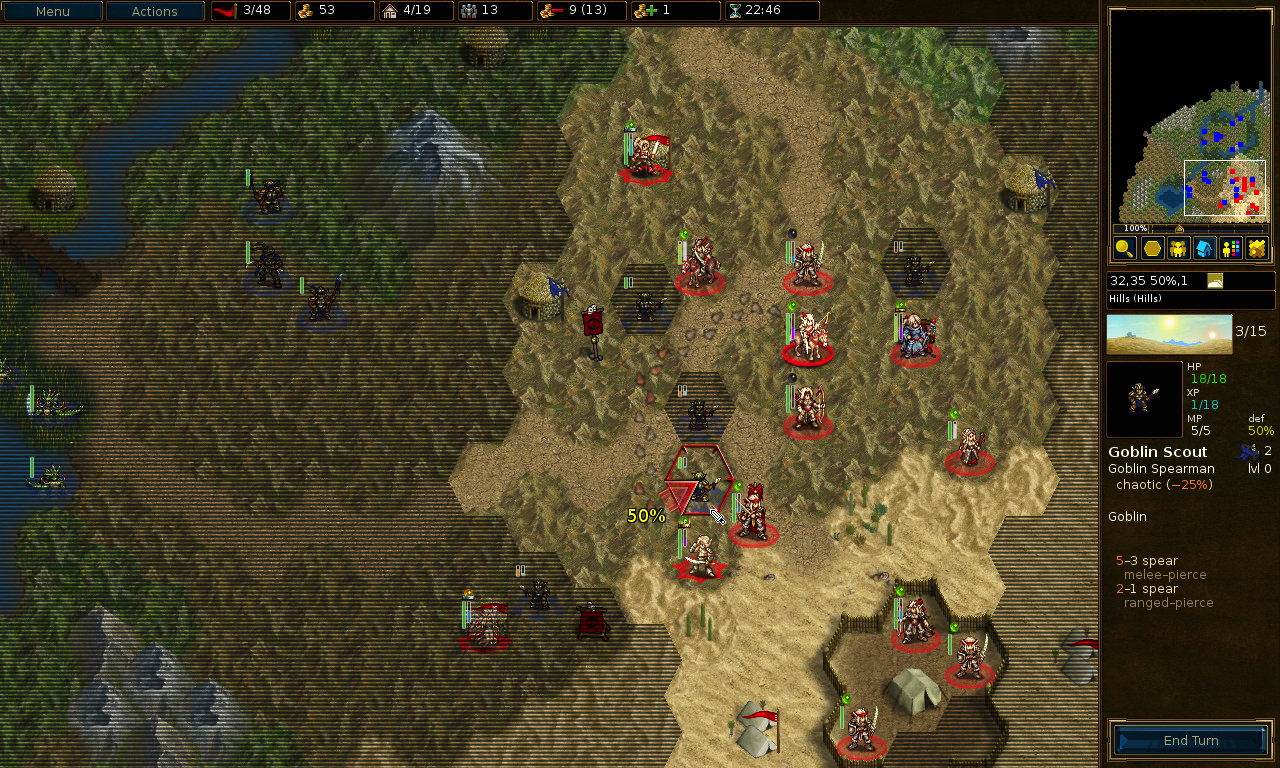
\includegraphics[width=1\textwidth]{figures/generating_levels/wesnoth_hex.png}
    \caption{Battle of Wesnoth, using a hexagonal tiling technique}\label{fig:wesnoth_hex} 
\end{figure}

Since the individual techniques mostly impact the visual appearance of the game
- the underlying data structures remain the same - we have chosen the apply the
most straightforward tiling technique: square tiles.
\\
\\
The first naive implementation we prototyped was to iterate through the
two-dimensional map and place tiles corresponding to the values, with tiles
being \texttt{sprites} in the gameworld. Sprites need to be assigned a
\texttt{sprite renderer} component which in turn needs to be attached a
\texttt{gameobject}. This effectively means that for each tile, we instantiate
a gameobject.  But since tiles exhibit no particular behavior, it seems
excessive to instantiate gameobjects for each tile. Not only that, but we were
experiencing performance implications on mobile devices using this method.  We
can substantially reduce the gameobjects required to be instantiated by
\textit{grouping} similar areas into bigger tiles. We do so by first
manipulating the data map such that we mark large areas, consisting of only one
type. We then \textit{blit} the texture associated with that type in a
tile-pattern, onto a bigger texture.  There is a technical limit to this
technique however, as texture-resolutions are limited by hardware. For our
particular implementation, we limit the resolution to 1024x1024 pixels, which
is within the limits of our target hardware. A comparison of the result of the
two techniques can be seen in figure~\ref{fig:grouped_tiling_comparison}.

\begin{figure}[H]
    \centering
    \begin{tabular}{cc}
        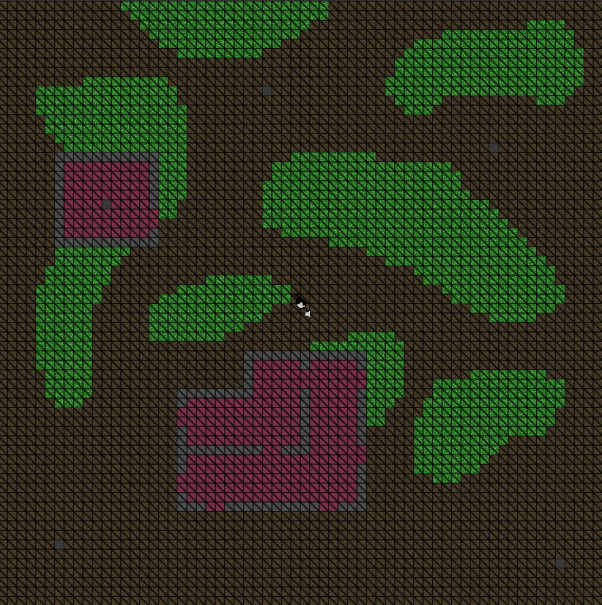
\includegraphics[width=0.5\textwidth]{figures/generating_levels/naive-tile.png}
        &
        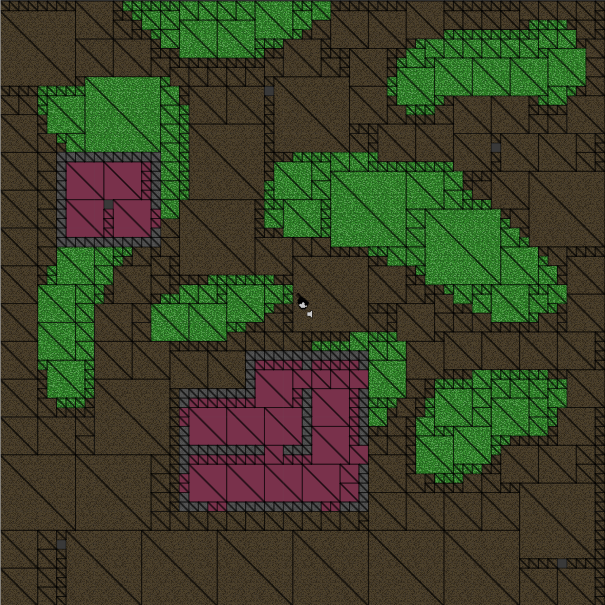
\includegraphics[width=0.5\textwidth]{figures/generating_levels/grouped-tile.png}
    \end{tabular}
    \caption{(left) naive tiling, (right) grouping tiles into larger tiles}\label{fig:grouped_tiling_comparison}
\end{figure}

The blitting is performed during runtime whenever a map is loaded, but in order
to avoid blitting the same texture - w.r.t. size and kind - more than once, we
cache the larger tiles to disk such that they can be loaded between subsequent
runs of the application. The performance overhead of blitting \textit{can} be
significant on mobile devices, as the larger textures have to be uploaded to
the GPU in order to reflect changes, and we did see improvements in that regard
by caching the blitted textures.
\\
\\
We also wanted \textit{transition} tiles between certain type of tiles, in
particular between grass and ground (this technique is also used in the games
seen in
figures~\ref{fig:civ-1_square},~\ref{fig:civ-2_iso}~and~\ref{fig:wesnoth_hex}).
We do so by using an adaptation of the \textit{Marching squares} algorithm, and
mark a position in the map as a particular type, based on the values of its
neighbors. A corresponding \textit{transition tile} is then blitted together
(and cached to disk in the same manner as grouped tiles), and assigned to it.
Figure~\ref{fig:transition_comparison} shows a comparison before and after
integrating the algorithm.
\todobrian{add ref for marching squares}

\begin{figure}[H]
    \centering
    \begin{tabular}{cc}
        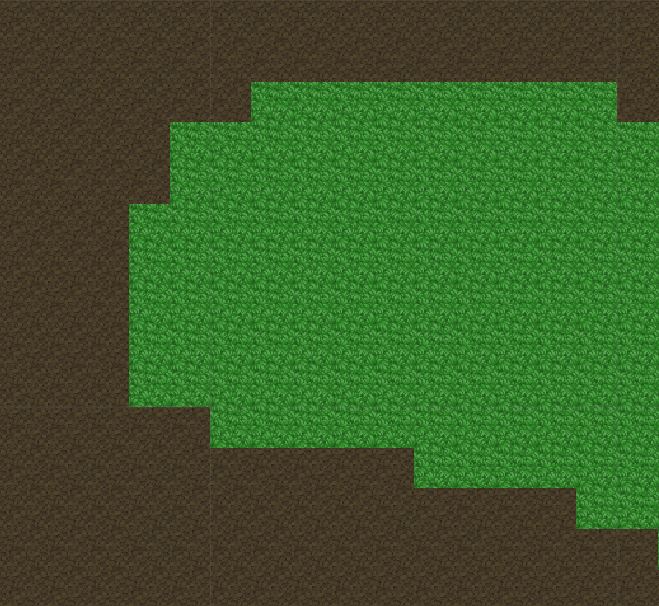
\includegraphics[width=0.5\textwidth]{figures/generating_levels/no_transition.png}
        &
        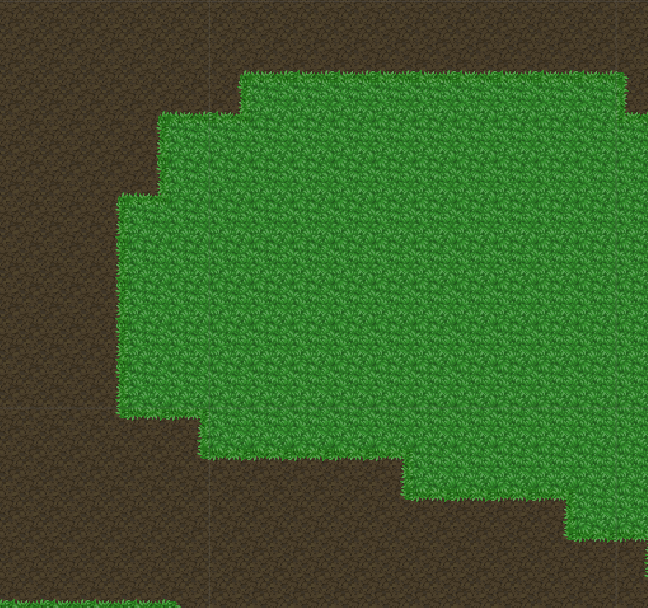
\includegraphics[width=0.5\textwidth]{figures/generating_levels/with_transition.png}
    \end{tabular}
    \caption{(left) without transitioning, (right) with transitioning tiles}\label{fig:transition_comparison}
\end{figure}

\section{Placing walls and colliders}
Placing walls involves both placing them as textured tiles within the
gameworld, and placing colliders such that players and NPC's cannot move
through them.

\subsection{Placing wall sprites}
A naive implementation for placing wallsprites within the gameworld is to place
a gameobject with the texture of a wall. However, we want our walls to look
``connected'' as if constructed together as on homogeneous unit. We do so by
using an adaptation of the \textit{Marching squares} (as we do with
transitional tiles between grass and ground). We can then detect if a wall is a
``stump'', a regular vertical or horizontal middle section or a t-section. We
do not allow for diagonal walls, so our marching squares adaptation only
considers adjacent tiles at 90-degree angles. Figure~\ref{fig:wall_comparison}
shows an example of placing walls where tiles are ``connected'' and one where
tiles are ``connected'' and figure~\ref{fig:walls_ingame} showing an in-game
example.

\begin{figure}[H]
    \centering
    \begin{tabular}{cc}
        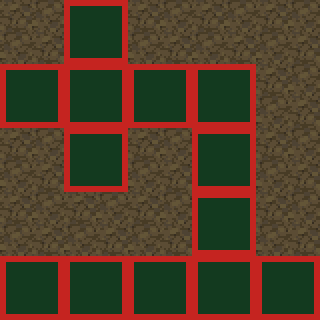
\includegraphics[width=0.5\textwidth]{figures/generating_levels/wall_no_border.png}
        &
        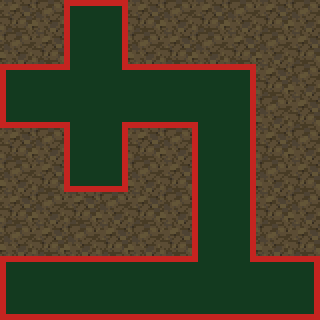
\includegraphics[width=0.5\textwidth]{figures/generating_levels/wall_with_border.png}
    \end{tabular}
    \caption{(left) not connected, and (right) where walls are connected}\label{fig:wall_comparison}
\end{figure}

\begin{figure}[H]
    \centering
    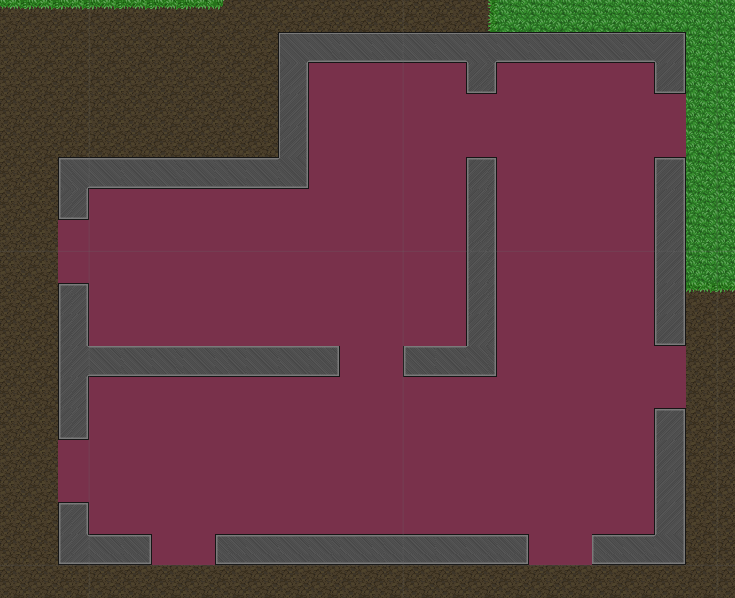
\includegraphics[width=1\textwidth]{figures/generating_levels/walls_ingame.png}
    \caption{In-game example of connected walls}\label{fig:walls_ingame} 
\end{figure}

\subsection{Placing wall colliders}
For wall colliders we want to \textit{translate} the contour of walls into
gameobjects assigned a collide-able component in the gameworld. The first naive
implementation we attempted was to place a square collider (regular
\texttt{Collider2D}) for each wall tile.
The positions for these colliders is shown as red dots in
figure~\ref{fig:wall_with_vertices}.
This resulted in the unfortunate behaviour that collisions from rigid bodies -
the player and enemies - behaved unreliable and rigid bodies would ``bounce off''
the walls whenever they would be ``between'' two collider sections.
\\
Our next idea was to find offsets for countour vertices for each tile, and
placing \texttt{Polygon Collider2D}, contour vertices shown as blue in
figure~\ref{fig:wall_with_vertices}. However this reveals a problem: the resulting
polygon we are interrested in is concave. This means that we cannot
\textit{easily} construct the polygon from only knowing the vertices. Our
solution was to use an adaptation of \textit{flood fill} to first find
connected vertical and then horizontal wall sections. From the algorithm, we
can find vertices for and construct concave polygons which are \textit{larger}
than single wall sections. This significantly reduces the number of colliders
necessary, almost eliminates the mentioned problem of unreliable behavior for
rigid bodies colliding with walls. An \textit{optimal} solution would be to
construct a concave polygon from the vertices, which would require finding all
countour vertices \textit{and} the order in which they should connected when
constructing the polygon. The result of our \textit{flood fill} approach can be
seen in figure~\ref{fig:wall_with_convex}.

\begin{figure}[H]
    \centering
    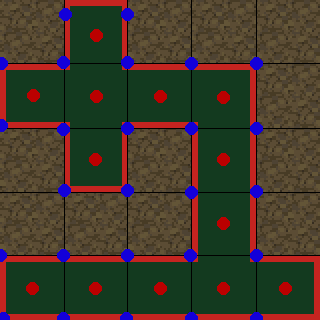
\includegraphics[width=1\textwidth]{figures/generating_levels/wall_with_vertices.png}
    \caption{Finding contour vertices}\label{fig:wall_with_vertices} 
\end{figure}

\begin{figure}[H]
    \centering
    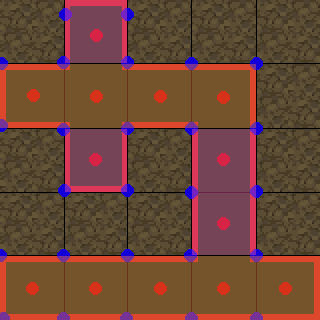
\includegraphics[width=1\textwidth]{figures/generating_levels/wall_with_convex.png}
    \caption{Finding connected concave polygons using flood fill}\label{fig:wall_with_convex} 
\end{figure}
